\documentclass{report}
\usepackage{homework}
\usepackage{graphicx}
\solstrue

\definecolor{mygray}{gray}{0.95}
\usepackage{listings}
\lstset{
basicstyle=\small\ttfamily,
columns=flexible,
breaklines=true,
backgroundcolor = \color{mygray},
framexleftmargin = 1em,
xleftmargin = 1em
}

\renewcommand{\hmwkTitle}{Homework 5}

\begin{document}
\mktitle


\begin{problem}
\begin{figure}[!ht]
	\centering
	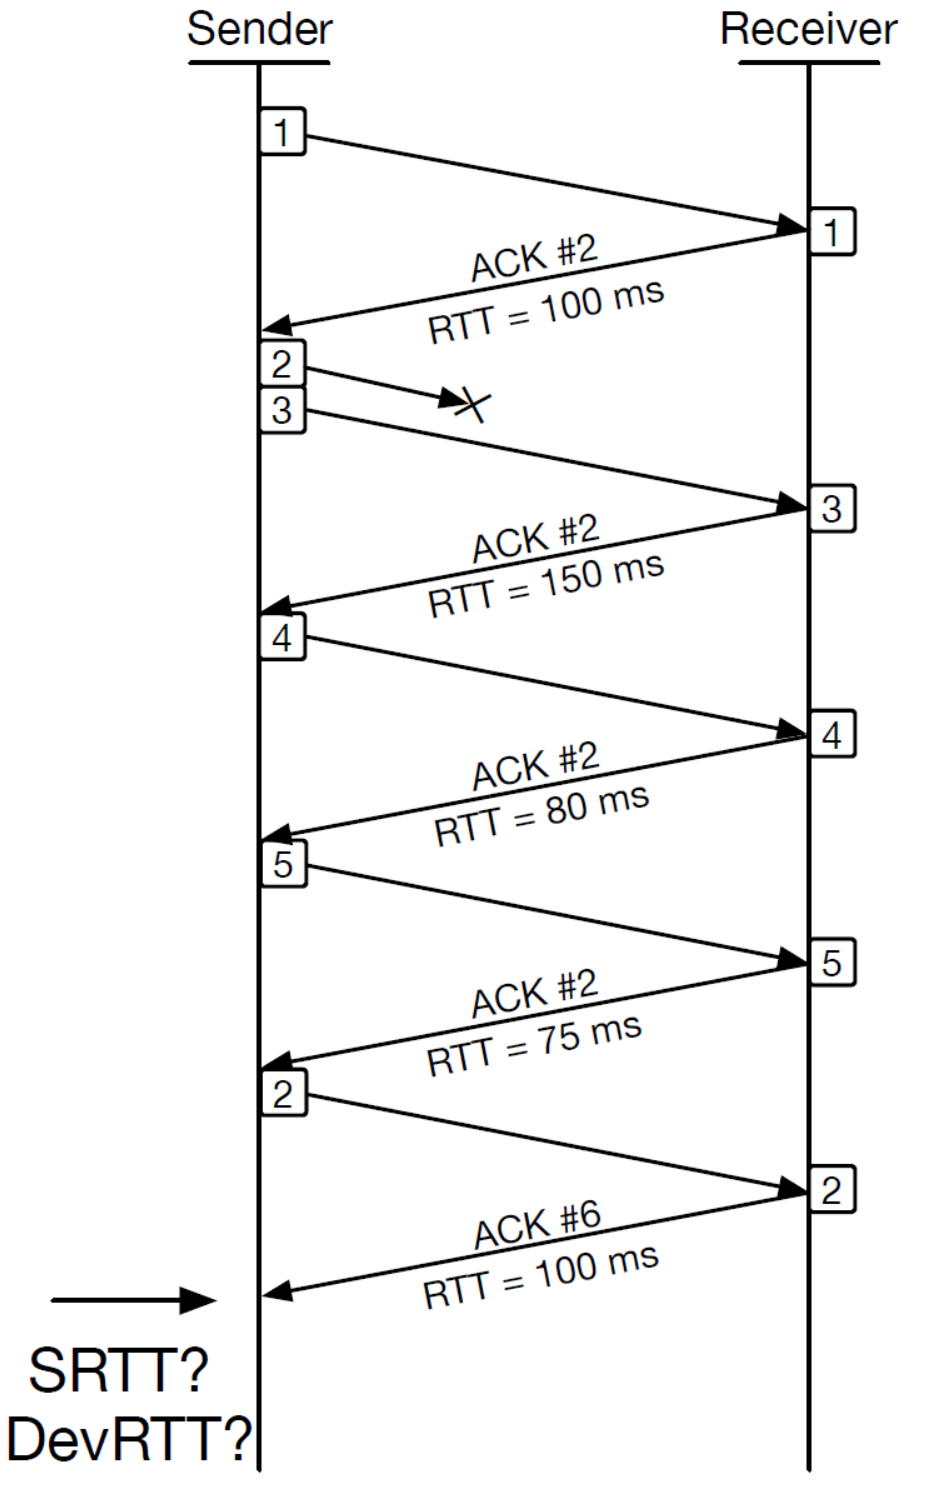
\includegraphics[width=0.5\textwidth]{image1.png}
	\caption{ TCP RTT estimation.}
	\centering
	\label{fig:image1}
\end{figure}

Calculate SRTT (RTT estimate), DevRTT, and RTO for a TCP connection shown in Figure 1 \textbf{at the marked point of time}. Use standard initial default parameters for the TCP connection (3 second for SRTT, 3 seconds for DevRTT), and α = 1/8, β = 1/4.\\
\indent Note that the second packet gets dropped during transmission and retransmitted at a later time.
\begin{enumerate}
	\item SRTT = 
	\item DevRTT = 
	\item RTO =
\end{enumerate}

\end{problem}

\clearpage
\begin{problem}

\begin{figure}[!ht]
	\centering
	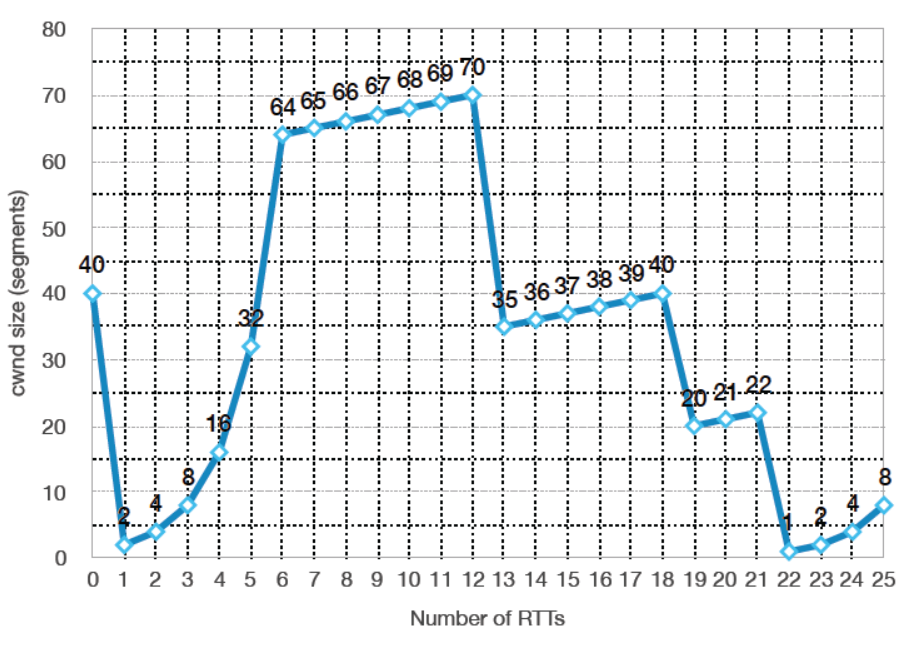
\includegraphics[width=0.5\textwidth]{image2.png}
	\caption{TCP congestion control.}
	\centering
	\label{fig:image2}
\end{figure}

Assume TCP Reno (with Fast Retransmit and Fast Recovery) is the protocol experiencing the behavior shown above. Assume that the TCP flow has been operating for some time, meaning that the number of RTTs shown are with respect to when you started observing the flows behavior.

\begin{enumerate}
\item \textbf{On the graph above}, identify the time periods when TCP slow start is operating.
\item \textbf{On the graph above}, identify the time periods when TCP congestion avoidance is operating (AIMD).
\item For each loss event, specify whether it was detected by a triple duplicate ACK or by a timeout
\item For each loss event, indicate the value of the slow start threshold (ssthresh)
\end{enumerate}

\begin{answer}{25em}

\end{answer}

\end{problem}

\clearpage
\begin{problem}

Consider transferring a large amount of data over the link with 10 Mbit/s bandwidth using TCP Reno (only you're using the link at this time). Assuming that losses in this link can only happen because of the buffer overflow, i.e., there are no random losses.
\begin{enumerate}
	\item Draw a diagram showing (approximately) how the sender’s cwnd changes over time.
	\item What is the maximum average throughput that this TCP flow can achieve?
\end{enumerate}

\begin{answer}{40em}
\end{answer}

\end{problem}


\clearpage
\begin{problem}

Suppose that two hosts are using TCP to communicate. They open a TCP connection between them and start to send data. Assume that \texttt{ssthresh} is 64 KB and the segment size is 3 KB.
\begin{enumerate}
	\item How many bytes are transmitted after 3 RTTs assuming no losses? Show your work.
	\item Now, suppose that after the third RTT, a loss occurs which results in the TCP sender timing out. What actions does TCP congestion control take?
	\item Assuming no losses will occur from then on, how many RTTs does it take to transmit an additional 22 KB of data?
\end{enumerate}

\begin{answer}{35em}
\end{answer}

\end{problem}


\end{document}
